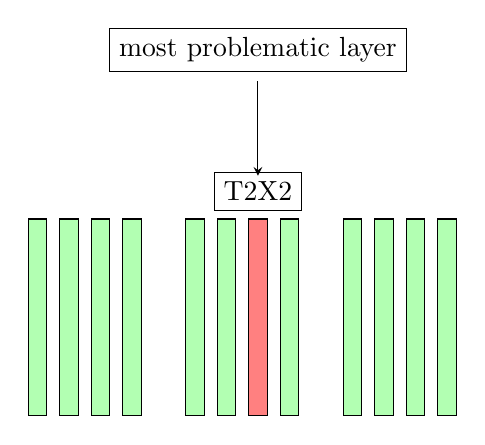
\begin{tikzpicture}

% first station
  \node[rectangle,
      draw = black,
      % text = ,
      fill = green!30!white,
      minimum width = 0.2cm,
      minimum height = 2.5cm] (r) at (0,0) {};

  \node[rectangle,
      draw = black,
      % text = ,
      fill = green!30!white,
      minimum width = 0.2cm,
      minimum height = 2.5cm] (r) at (0.4,0) {};

  \node[rectangle,
      draw = black,
      % text = ,
      fill = green!30!white,
      minimum width = 0.2cm,
      minimum height = 2.5cm] (r) at (0.8,0) {};

  \node[rectangle,
      draw = black,
      % text = ,
      fill = green!30!white,
      minimum width = 0.2cm,
      minimum height = 2.5cm] (r) at (1.2,0) {};

% second station
  \node[rectangle,
      draw = black,
      % text = ,
      fill = green!30!white,
      minimum width = 0.2cm,
      minimum height = 2.5cm] (r) at (2,0) {};

  \node[rectangle,
      draw = black,
      % text = ,
      fill = green!30!white,
      minimum width = 0.2cm,
      minimum height = 2.5cm] (r) at (2.4,0) {};

  \node[rectangle,
      draw = black,
      % text = ,
      fill = red!50!white,
      minimum width = 0.2cm,
      minimum height = 2.5cm] (r) at (2.8,0) {};
\node[draw, align=left] at (2.8, 1.6) {T2X2}; % node for bad layer
\draw[-stealth] (2.8,3.0) -- (2.8,1.8); % draw arrow to bad layer
\node[draw, align=left] at (2.8, 3.4) {most problematic layer}; % make node above layer

  \node[rectangle,
      draw = black,
      % text = ,
      fill = green!30!white,
      minimum width = 0.2cm,
      minimum height = 2.5cm] (r) at (3.2,0) {};

  % third station
    \node[rectangle,
        draw = black,
        % text = ,
        fill = green!30!white,
        minimum width = 0.2cm,
        minimum height = 2.5cm] (r) at (4,0) {};

    \node[rectangle,
        draw = black,
        % text = ,
        fill = green!30!white,
        minimum width = 0.2cm,
        minimum height = 2.5cm] (r) at (4.4,0) {};

    \node[rectangle,
        draw = black,
        % text = ,
        fill = green!30!white,
        minimum width = 0.2cm,
        minimum height = 2.5cm] (r) at (4.8,0) {};

    \node[rectangle,
        draw = black,
        % text = ,
        fill = green!30!white,
        minimum width = 0.2cm,
        minimum height = 2.5cm] (r) at (5.2,0) {};
\end{tikzpicture}
